%%
%% If your work has an appendix, this is the place to put it.
\appendix

\section{Common Elements}

\subsection{Tables}

The ``\verb|acmart|'' document class includes the ``\verb|booktabs|''
package --- \url{https://ctan.org/pkg/booktabs} --- for preparing
high-quality tables.

Table captions are placed {\itshape above} the table.

Because tables cannot be split across pages, the best placement for
them is typically the top of the page nearest their initial cite.  To
ensure this proper ``floating'' placement of tables, use the
environment \textbf{table} to enclose the table's contents and the
table caption.  The contents of the table itself must go in the
\textbf{tabular} environment, to be aligned properly in rows and
columns, with the desired horizontal and vertical rules.  Again,
detailed instructions on \textbf{tabular} material are found in the
\textit{\LaTeX\ User's Guide}.

Immediately following this sentence is the point at which
Table~\ref{tab:freq} is included in the input file; compare the
placement of the table here with the table in the printed output of
this document.

\begin{table}[h]
  \caption{Frequency of Special Characters}
  \label{tab:freq}
  \centering
  \begin{tabular}{ccl}
    \toprule
    Non-English or Math&Frequency&Comments\\
    \midrule
    \O & 1 in 1,000& For Swedish names\\
    $\pi$ & 1 in 5& Common in math\\
    \$ & 4 in 5 & Used in business\\
    $\Psi^2_1$ & 1 in 40,000& Unexplained usage\\
  \bottomrule
\end{tabular}
\end{table}

To set a wider table, which takes up the whole width of the page's
live area, use the environment \textbf{table*} to enclose the table's
contents and the table caption.  As with a single-column table, this
wide table will ``float'' to a location deemed more
desirable. Immediately following this sentence is the point at which
Table~\ref{tab:commands} is included in the input file; again, it is
instructive to compare the placement of the table here with the table
in the printed output of this document.

\begin{table*}
  \caption{Some Typical Commands}
  \label{tab:commands}
  \centering
  \begin{tabular}{ccl}
    \toprule
    Command &A Number & Comments\\
    \midrule
    \texttt{{\char'134}author} & 100& Author \\
    \texttt{{\char'134}table}& 300 & For tables\\
    \texttt{{\char'134}table*}& 400& For wider tables\\
    \bottomrule
  \end{tabular}
\end{table*}

Always use midrule to separate table header rows from data rows, and
use it only for this purpose. This enables assistive technologies to
recognise table headers and support their users in navigating tables
more easily.

\subsection{Math Equations}
You may want to display math equations in three distinct styles:
inline, numbered or non-numbered display.  Each of the three are
discussed in the next sections.

\subsubsection{Inline (In-text) Equations}
A formula that appears in the running text is called an inline or
in-text formula.  It is produced by the \textbf{math} environment,
which can be invoked with the usual
\texttt{{\char'134}begin\,\ldots{\char'134}end} construction or with
the short form \texttt{\$\,\ldots\$}. You can use any of the symbols
and structures, from $\alpha$ to $\omega$, available in
\LaTeX~\cite{Lamport:LaTeX}; this section will simply show a few
examples of in-text equations in context. Notice how this equation:
\begin{math}
  \lim_{n\rightarrow \infty}x=0
\end{math},
set here in in-line math style, looks slightly different when
set in display style.  (See next section).

\subsubsection{Display Equations}
A numbered display equation---one set off by vertical space from the
text and centered horizontally---is produced by the \textbf{equation}
environment. An unnumbered display equation is produced by the
\textbf{displaymath} environment.

Again, in either environment, you can use any of the symbols and
structures available in \LaTeX\@; this section will just give a couple
of examples of display equations in context.  First, consider the
equation, shown as an inline equation above:
\begin{equation}
  \lim_{n\rightarrow \infty}x=0
\end{equation}
Notice how it is formatted somewhat differently in
the \textbf{displaymath}
environment.  Now, we'll enter an unnumbered equation:
\begin{displaymath}
  \sum_{i=0}^{\infty} x + 1
\end{displaymath}
and follow it with another numbered equation:
\begin{equation}
  \sum_{i=0}^{\infty}x_i=\int_{0}^{\pi+2} f
\end{equation}
just to demonstrate \LaTeX's able handling of numbering.

\subsection{Figures}

The ``\verb|figure|'' environment should be used for figures. One or
more images can be placed within a figure. If your figure contains
third-party material, you must clearly identify it as such, as shown
in the example below.
\begin{figure}[h]
  \centering
  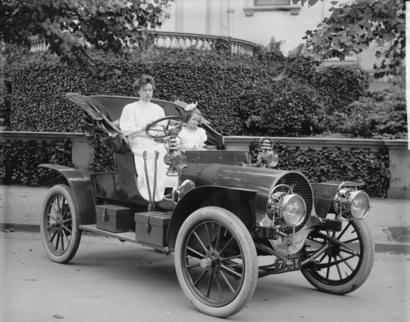
\includegraphics[width=\linewidth]{figures/sample-franklin.png}
  \caption{1907 Franklin Model D roadster. Photograph by Harris \&
    Ewing, Inc. [Public domain], via Wikimedia
    Commons. (\url{https://goo.gl/VLCRBB}).}
  \Description{A woman and a girl in white dresses sit in an open car.}
\end{figure}

Your figures should contain a caption which describes the figure to
the reader.

Figure captions are placed {\itshape below} the figure.

Every figure should also have a figure description unless it is purely
decorative. These descriptions convey what’s in the image to someone
who cannot see it. They are also used by search engine crawlers for
indexing images, and when images cannot be loaded.

A figure description must be unformatted plain text less than 2000
characters long (including spaces).  {\bfseries Figure descriptions
  should not repeat the figure caption – their purpose is to capture
  important information that is not already provided in the caption or
  the main text of the paper.} For figures that convey important and
complex new information, a short text description may not be
adequate. More complex alternative descriptions can be placed in an
appendix and referenced in a short figure description. For example,
provide a data table capturing the information in a bar chart, or a
structured list representing a graph.  For additional information
regarding how best to write figure descriptions and why doing this is
so important, please see
\url{https://www.acm.org/publications/taps/describing-figures/}.

\subsection{Code Snippet}

\begin{minted}[frame=single,framesep=10pt]{python}
# main notebook
foo = 123
\end{minted}
\begin{minted}[frame=single,framesep=10pt]{python}
# parallel cell group named 'plel'
foo = foo +  5
bar = 'hello'
foo # note: in "standard" Jupyter, this line outputs '128' when the user executes this cell
\end{minted}

